\documentclass[12pt,letterpaper]{article}
\usepackage{anysize}
\usepackage{amsmath}
\marginsize{2cm}{2cm}{1cm}{1cm}
\usepackage{listings}
\usepackage{cite}
\usepackage{caption}
\usepackage{upquote}
\usepackage{xcolor}
\usepackage{xcolor}

\usepackage{tikz}
\def\checkmark{\tikz\fill[scale=0.4](0,.35) -- (.25,0) -- (1,.7) -- (.25,.15) -- cycle;} 

\usepackage{graphicx}


\begin{document}

\begin{titlepage}
    \vspace*{4cm}
    \begin{flushleft}
    {\huge
        CS519 Project 8\\[.5cm]
    }
    {\large
        Dog Poster\\
		Dog and Black Hole
    }
    \end{flushleft}
    \vfill
    \rule{5in}{.5mm}\\
    Li Li

\end{titlepage}
\section{source files}
There are only three files dogmorph.frag, dogmorph.glib and dogmorph.vert. Also, I use updated dog2.obj file. Lastly, there is a all4.jpg that is reserved for poster.
\section{a simple explanation}
What I did are:\\
\begin{tabular}{ |l | c |}
  \hline                       
  \textbf{Feature} & \textbf{Status} \\ \hline
  Morphing dog base on distance to a black hole& \checkmark \\ \hline
  Getting rid of those pass the black hole& \checkmark \\ \hline
  Changing position of black hole& \checkmark \\ \hline
\end{tabular}

\begin{itemize}
\item For the this \textbf{Morphing}, I do make use of gravity formula: $F = Gm_{1}m_{2}/r^{2}$. In my function I input a uForce parameter to stand $Gm_{1}m_{2}$. It can be simply explained as: G is constant,$m_{1}$ is our dog(constant). Only the mass of $m_{2}$ varying that is our black hole. This \textit{r} is the distance from black hole(which is just a point) to a certain vertex of the dog. Now we got this \textit{F}. As \textit{F} (gravity) grows, dog morphs tremendously. So, it is a linear relationship between gravity and morphing. So just replace blend value with this \textit{F}. For mix function, we have one value is the pos of black hole, the other one is pos of a certain vertex of the dog.
\item For \textbf{deleting those passed the black hole}, I calculate two vectors. One is from newly morphed pos to black hole point, another is from old non-morphed pos to black hole point. If the dot product of thes two vector is above zero, I apply the morphing. Otherwise set the new pos as the pos of black hole point.
\item About \textbf{Changing pos of black hole}, setting uX,uY,uZ to adjust the pos of black hole this pos is in world coordinate.

\end{itemize}
\section{result}

\begin{figure}[p]
    \centering
    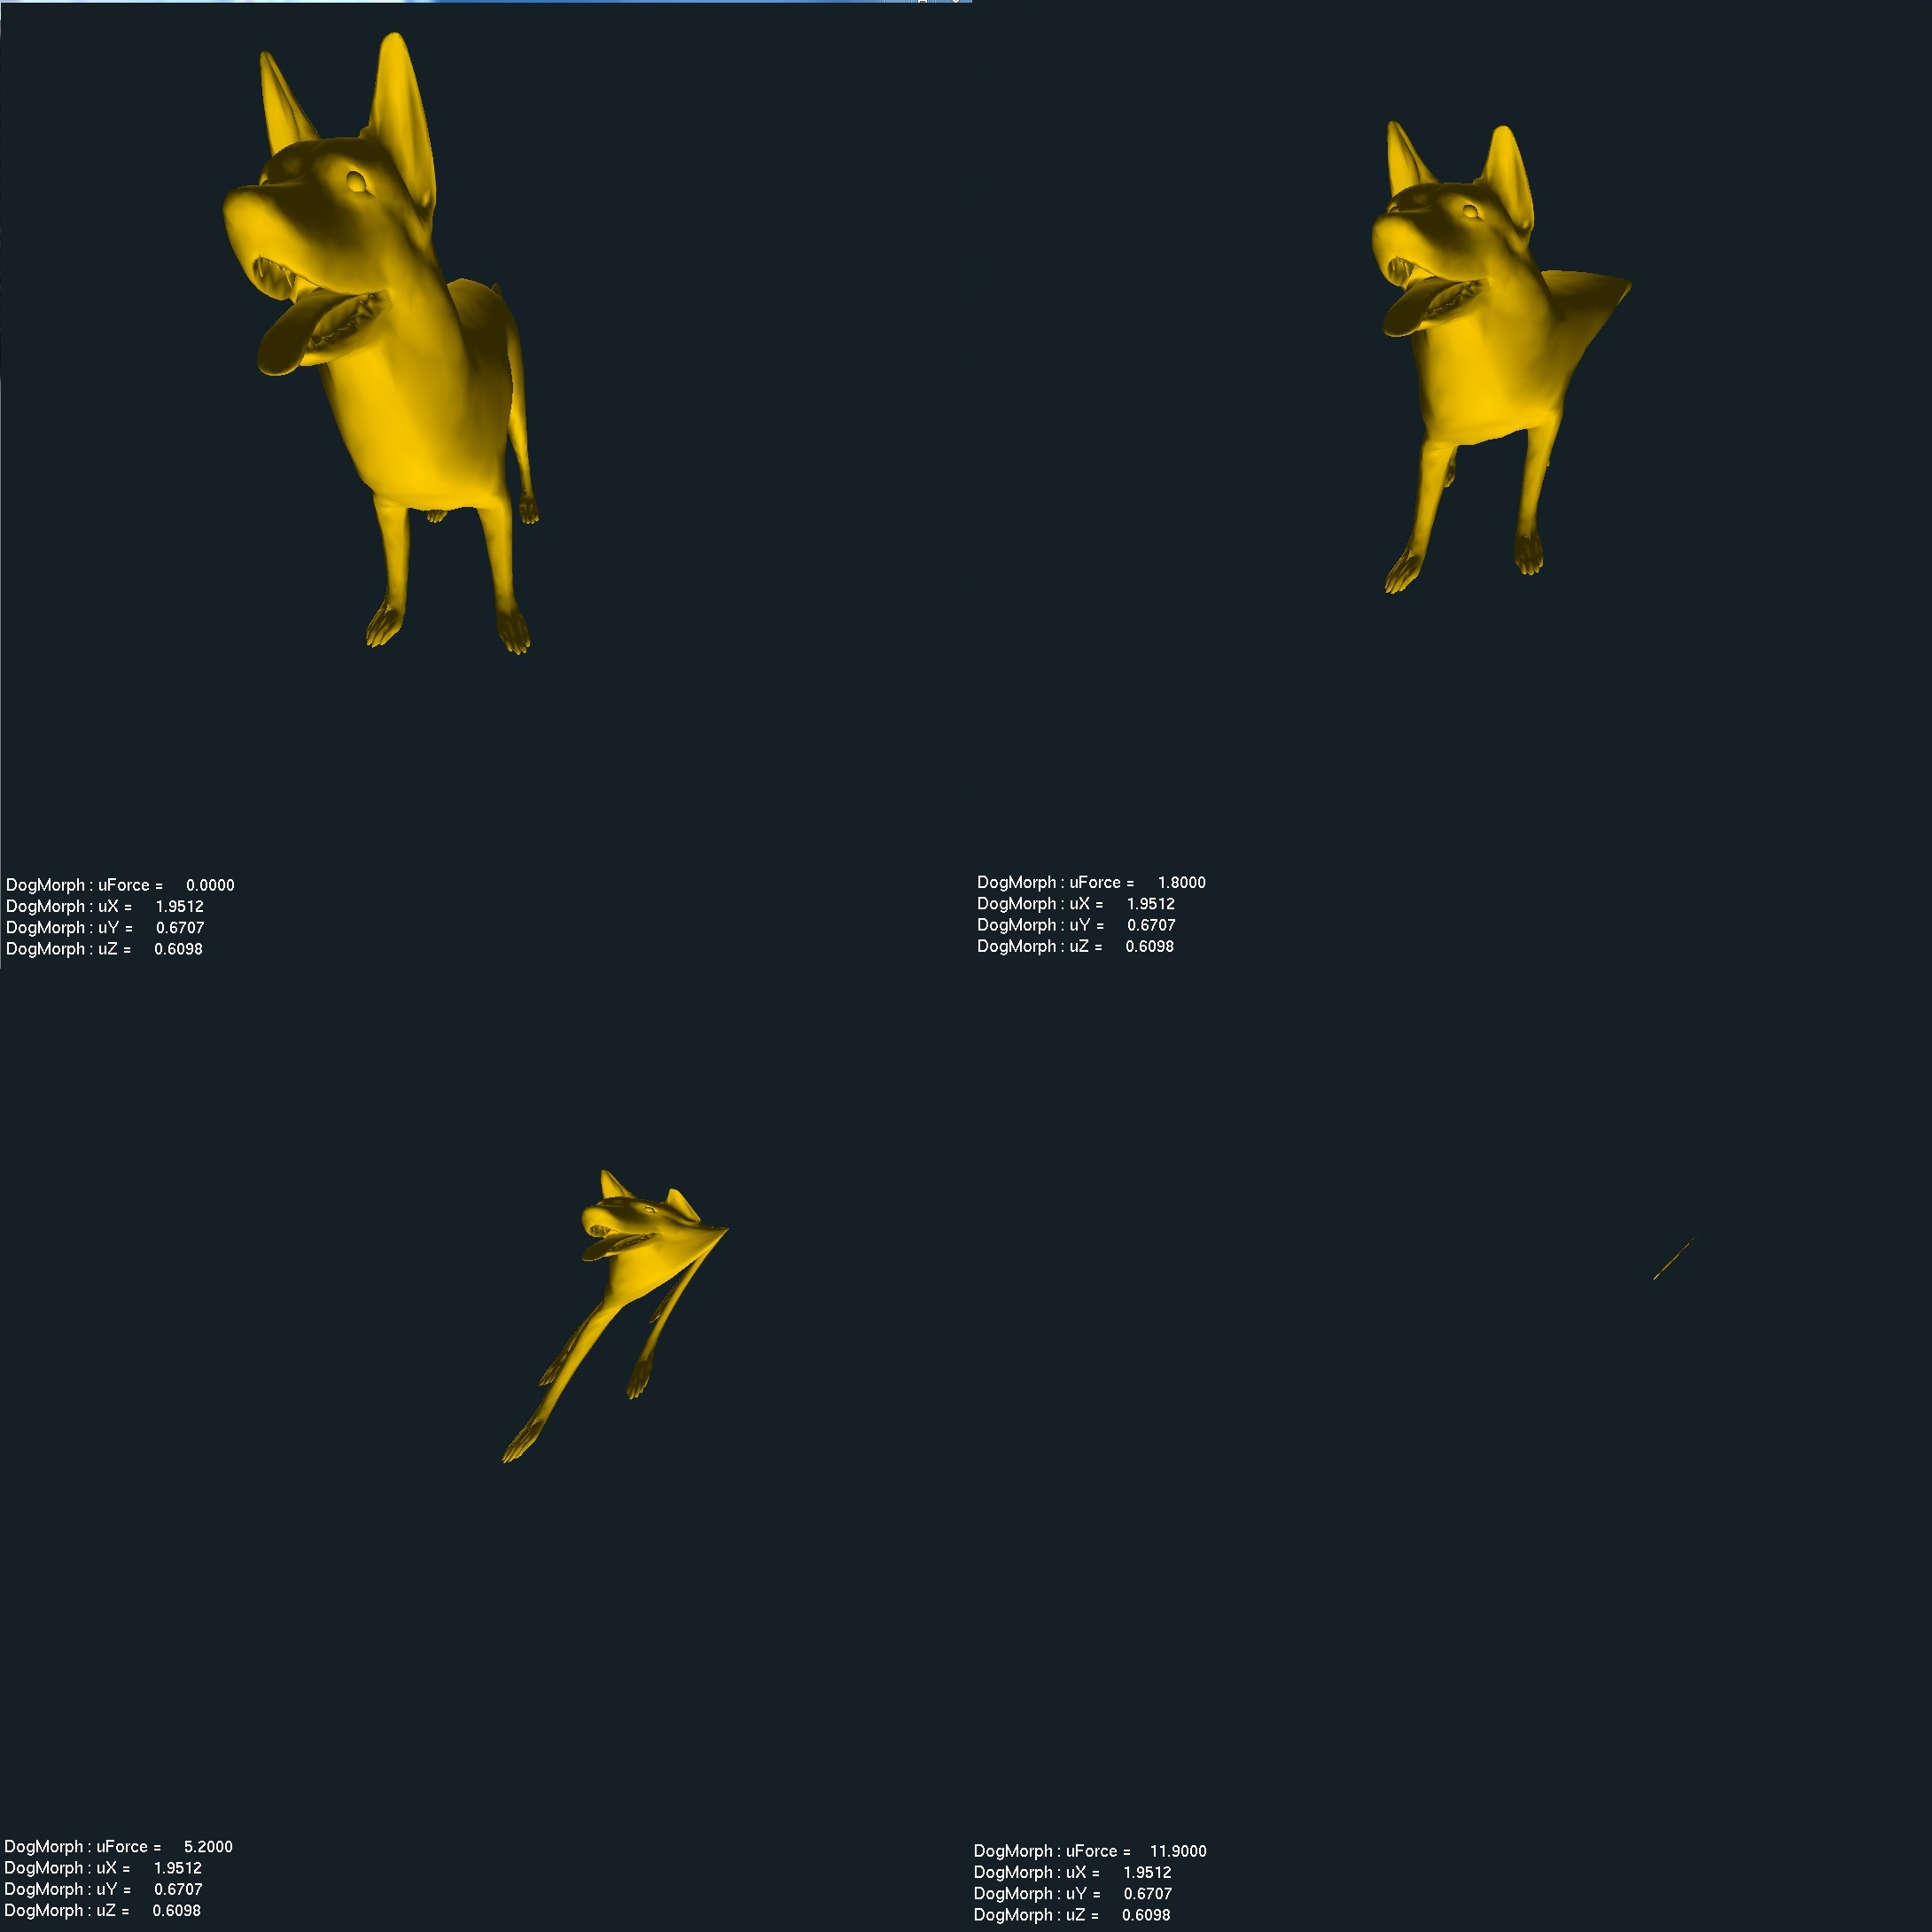
\includegraphics[width=1.0\textwidth]{all4.jpg}
    \caption{Dog from complete to disappear}
\end{figure}

\end {document}
